\documentclass[pdftex,11pt]{article}
\usepackage[pdftex]{graphicx}
\usepackage{enumerate}
\usepackage{amsmath}
\usepackage{amssymb}
\usepackage{multicol}
\usepackage{algpseudocode}
\usepackage{algorithm}

\begin{document}
\title{COMP 540 Statistical Machine Learning}
\author{Xiang Zhou (xz58) - Guangyuan Yu ()}
\date{2017.01.17}
\maketitle
\newcommand{\pr}{\mathbb{P}}

\section{Locally weighted linear regression}
\begin{itemize}
\item Part 1 \begin{align*}
	J(\theta)&=\sum^m_{i=1}w^{(i)}(\theta^Tx^{(i)}-y^{(i)})^2=(X\theta-y)^TW(X\theta-y)\\
	A&=X\theta-y=
	\begin{pmatrix}
		x_1^{(1)} & \cdots & x_D^{(1)}\\
		\vdots & \ddots & \vdots\\
		x_1^{(N)} & \cdots & x_D^{(N)}
	\end{pmatrix}\\
	J(\theta)&=A^TWA=(x^{(1)^T}-y^{(1)}\cdots x^{(N)^T}\theta-y^{(N)})
	\begin{pmatrix}
		w^{(1)} & \cdots & 0\\
		\vdots & \ddots & \vdots\\
		0 & \cdots & w^{(n)}
	\end{pmatrix}
	\begin{pmatrix}
		x^{(1)^T}\theta-y^{(1)}\\
		\vdots\\
		x^{(N)^T}\theta-y^{(N)}
	\end{pmatrix}\\
	&=\sum^m_{i=1}w^{(i)}(x^{(i)^T}\theta-y^{(i)})^2=w^{(i)}(\theta^Tx^{(i)}-y^{(i)})^2
	\end{align*}
\item Part 2 \begin{align*}
	J(\theta)&=(X\theta-y)^TW(X\theta-y)\\
	&=(\theta^TX^T-yT)W(X\theta-y)\\
	&=\theta^TX^TWX\theta-\theta^TX^TWXy-y^TWX\theta+y^TWy
	\end{align*}
	Because $(\theta^TX^TW)$ and $y$ are $1\times N$ and $N\times 1$ respectively, $\theta^TX^TWy=y^TWX\theta$.
	$$\frac{dJ(\theta)}{d\theta}=0=\frac{d}{d\theta}[\theta^TX^TWX\theta]-2\frac{d}{d\theta}[\theta^TX^TWy]+\frac{d}{d\theta}[y^TWy]$$
	By taking the matrix derivative, we get:
	$$0=2X^TWX\theta-2X^TWy$$
	$$\hat{\theta}=(X^TWX)^{-1}X^TWy$$
\item Part 3
\begin{algorithm}
  \caption{Calculating $\theta$ by Batch Gradient Descent}

  \begin{algorithmic}
  	\State {\em Input}: Data Matrix $X \in m\times d+1$, vector $y\in m\times 1$, learning rate $\alpha\in \mathbb{R}$, input vector $x\in\mathbb{R}^{d+1}$, bandwidth of sphere of influence around $x$ $\tau$
	\State {\em Output}: Vector $\theta\in\mathbb{R}^{d+1}$ that minimizes weighted LSE\\
	\State $w\gets m\times n$ zeros matrix
	\State $\theta\gets d\times 1$ zeros matrix
	\State $grad\gets d\times 1$ zeros matrix
	\For {$j=0$ to $m$}
	\State $w_j^{(j)}\gets\frac{(x-X^{(j)})^T(x-X^{(j)})}{2\tau^2}$
	\EndFor
	\For {$j=0$ to $5000$} \Comment{arbitrary number of iterations}
	\State $grad\gets\frac{X^Tw(X\theta-y)}{m}$
	\State $\theta\gets\theta-\alpha*grad$
	\EndFor
	\State \Return $\theta$
  \end{algorithmic}
\end{algorithm}
\end{itemize}

\section{Properties of the linear regression estimator}
\begin{itemize}
\item Under the assumption that $E[\epsilon]=0$,
	\begin{align*}
		\theta&=(X^TX)^{-1}X^Ty\\
		E[\theta]&=E[(X^TX)^{-1}X^Ty]\\
		&=(X^TX)^{-1}X^TE[X\theta^*+\epsilon]\\
		&=(X^TX)^{-1}(X^TX)\theta^*+(X^TX)^{-1}X^TE[\epsilon]\\
		&=\theta^*+0=\theta^*
	\end{align*}
\item Under the assumption that $Var(\epsilon)=\sigma^2$,
	\begin{align*}
		Var(\theta)&=Var((X^TX)^{-1}X^Ty)\\
		&=Var((X^TX)^{-1}X^T(X\theta^*+\epsilon))\\
		&=Var(\theta^*)+Var((X^TX)^{-1}\epsilon)\\
		&=0+(X^TX)^{-1}Var(\epsilon)\\
		&=(X^TX)^{-1}\sigma^2
	\end{align*}
\end{itemize}

\section{Implementing linear regression and regularized linear regression}
\subsection{Implementing linear regression}
\subsubsection{Linear regression with one variable}
Prediction of 5\% LSTAT: 298224.50151\\
Prediction of 50\% LSTAT: -5787.31930418

\subsubsection{Linear regression with multiple variables}
\begin{itemize}
\item Prediction of 'average tract': 225328.063241
\item The predictions using gradient descent and the normal equation match up. The LSE we're minimizing has a unique minimum that both methods find. The $\theta$s provided for the two solutions were different, and this is due to the fact that we normalized the feature data for the gradient descent.
\item After running the four different learning rates provided (.01, .03, .1, and .3), we found that all converged, none with oscillation, on the same value. Thus, the best choice for a learning rate out of these four is 0.3 due to the fact that it converges the fastest and thus requires the least amount of iterations to finish training. We went a step further and increased the scale logarithmically again, testing out learning rates = \{1,3\}. Here I ran into issues where the loss climbed incredibly until it reached NAN by the 300th iteration and 200th iteration with 1 and 3 respectively. Thus, we found that .3 is the most suitable learning rate. See Figures \ref{fig:lr001}-\ref{fig:lr3}.
\end{itemize}

\subsection{Implementing regularized linear regression}
\begin{itemize}
\item As $\lambda$ increases, the fit becomes resistant to changes to $\theta$. We decrease variance and increase bias, so the shape of the fit becomes more regular and less curvy. Because of this, the training error constant increases. Validation error decreases from $\lambda=0$, but then begins to increase as our bias becomes greater and we make more assumptions about the fit that we shouldn't be making. See Figures \ref{fig:fit1}-\ref{fig:learn100}
\item Based on our error curve, We find a clear minimum between $0.1$ and $1$. Give our $\lambda$ range, we conclude that $0.3$ is the best choice of $\lambda$ for this problem. It is also interesting to note that this gives us the highest training error. See Figure \ref{fig:bestlambda}
\item Test error: 4.68\\Based on the error curve from the previous part, this is a good error compared to the validation and training error using our optimal $\lambda$. 
\end{itemize}


%commneted
\iffalse
\pagebreak
\section*{Appendix}
\begin{figure}[H]
  \caption{Learning rate = 0.01}
  \label{fig:lr001}
  \centering
    \includegraphics[scale=0.5]{part1/lr0.pdf}
\end{figure}
\begin{figure}[H]
  \caption{Learning rate = 0.03}
  \centering
    \includegraphics[scale=0.5]{part1/lr1.pdf}
\end{figure}
\begin{figure}[H]
  \caption{Learning rate = 0.1}
  \centering
    \includegraphics[scale=0.55]{part1/lr2.pdf}
\end{figure}
\begin{figure}[H]
  \caption{Learning rate = 0.3}
  \centering
    \includegraphics[scale=0.55]{part1/lr3.pdf}
\end{figure}
\begin{figure}[H]
  \caption{Learning rate = 1}
  \centering
    \includegraphics[scale=0.55]{part1/lr4.pdf}
\end{figure}
\begin{figure}[H]
  \caption{Learning rate = 3}
  \label{fig:lr3}
  \centering
    \includegraphics[scale=0.55]{part1/lr5.pdf}
\end{figure}

% part 2
\begin{figure}[H]
  \caption{Training data for regularized linear regression}
  \centering
    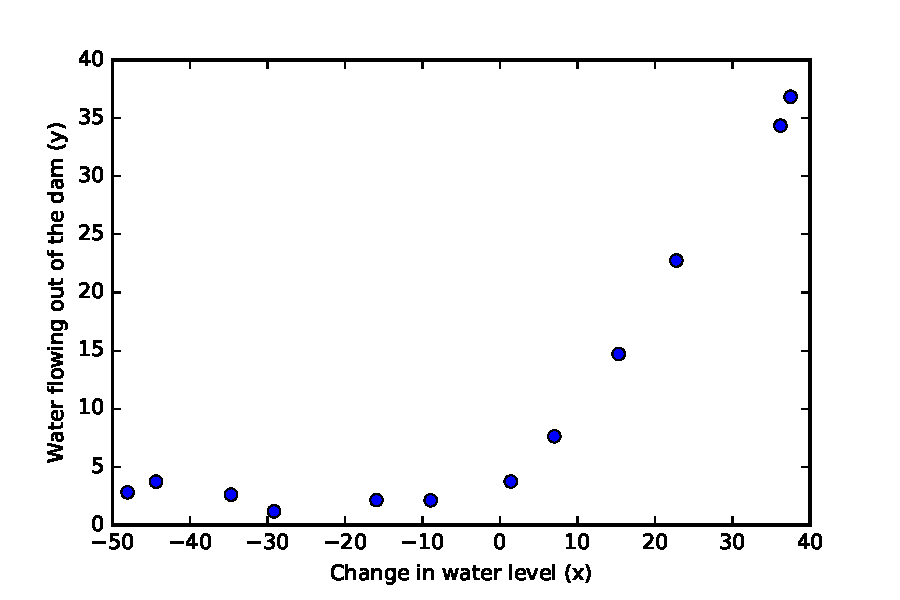
\includegraphics[scale=0.55]{part2/fig6.pdf}
\end{figure}
\begin{figure}[H]
  \caption{Best fit line for training data}
  \centering
    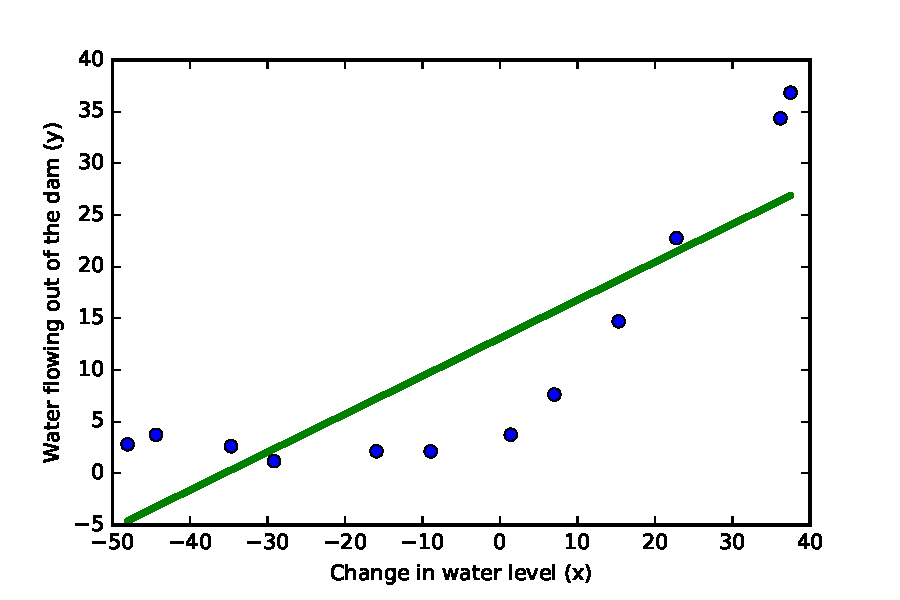
\includegraphics[scale=0.55]{part2/fig7.pdf}
\end{figure}
\begin{figure}[H]
  \caption{Learning curve for linear regression, $\lambda=0$}
  \centering
    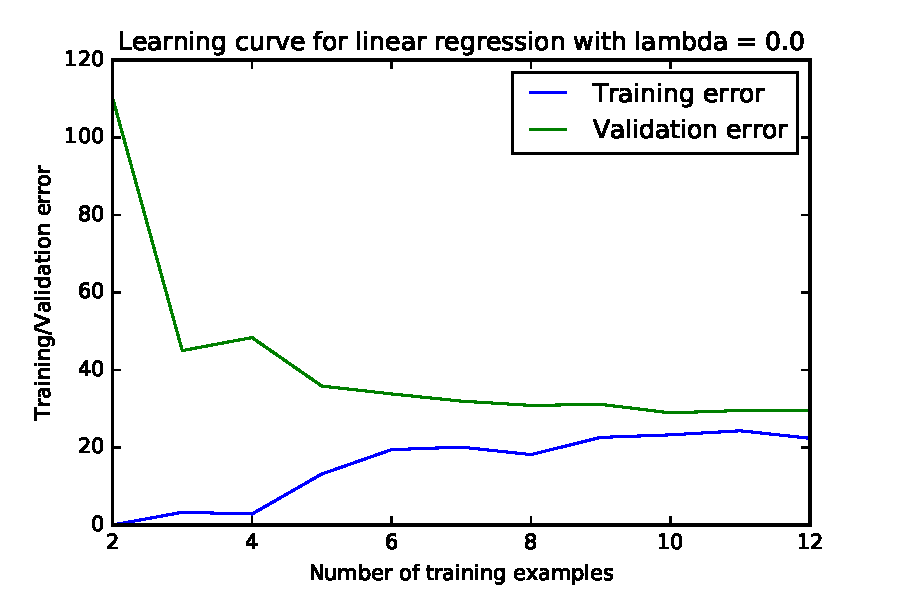
\includegraphics[scale=0.55]{part2/fig8.pdf}
\end{figure}

\pagebreak
\begin{figure}[H]
  \caption{Polynomial fit for $\lambda=0$ and $p=6$}
  \centering
    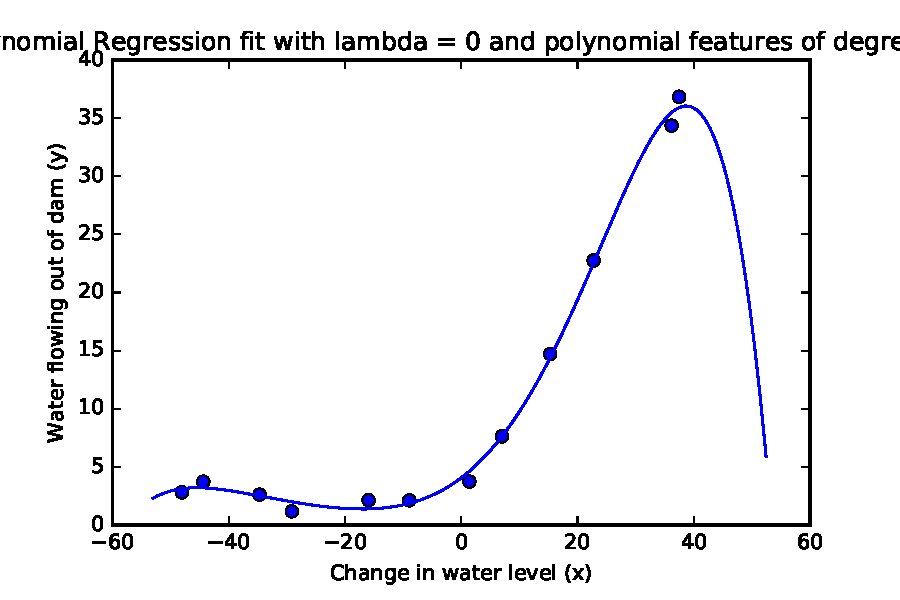
\includegraphics[scale=0.55]{part2/fig9.pdf}
\end{figure}
\begin{figure}[H]
  \caption{Learning curve for $\lambda=0$}
  \centering
    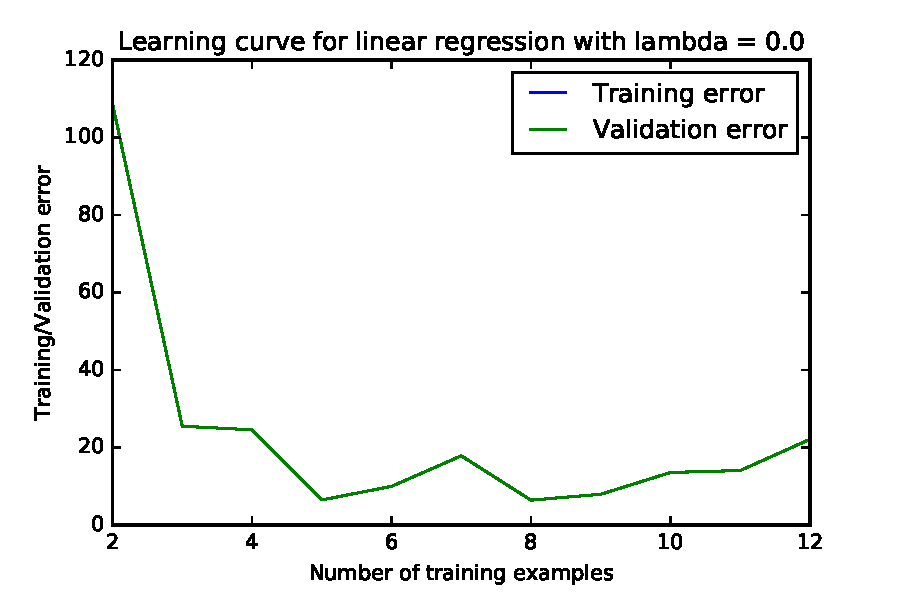
\includegraphics[scale=0.55]{part2/fig10.pdf}
\end{figure}
\begin{figure}[H]
\caption{Polynomial fit for $\lambda=1$ and $p=6$}
\label{fig:fit1}
  \centering
\includegraphics[scale=0.55]{part2/fit1.pdf}
\end{figure}
\begin{figure}[H]
\caption{Learning curve for $\lambda=1$}
  \centering
\includegraphics[scale=0.55]{part2/learn1.pdf}
\end{figure}
\begin{figure}[H]
\caption{Polynomial fit for $\lambda=10$ and $p=6$}
  \centering
\includegraphics[scale=0.55]{part2/fit10.pdf}
\end{figure}
\begin{figure}[H]
\caption{Learning curve for $\lambda=10$}
  \centering
\includegraphics[scale=0.55]{part2/learn10.pdf}
\end{figure}
\begin{figure}[H]
\caption{Polynomial fit for $\lambda=100$ and $p=6$}
  \centering
\includegraphics[scale=0.55]{part2/fit100.pdf}
\end{figure}
\begin{figure}[H]
\caption{Learning curve for $\lambda=100$}
  \label{fig:learn100}
  \centering
\includegraphics[scale=0.55]{part2/learn100.pdf}
\end{figure}


\begin{figure}[H]
\caption{Learning curves for different $\lambda$s}
  \label{fig:bestlambda}
  \centering
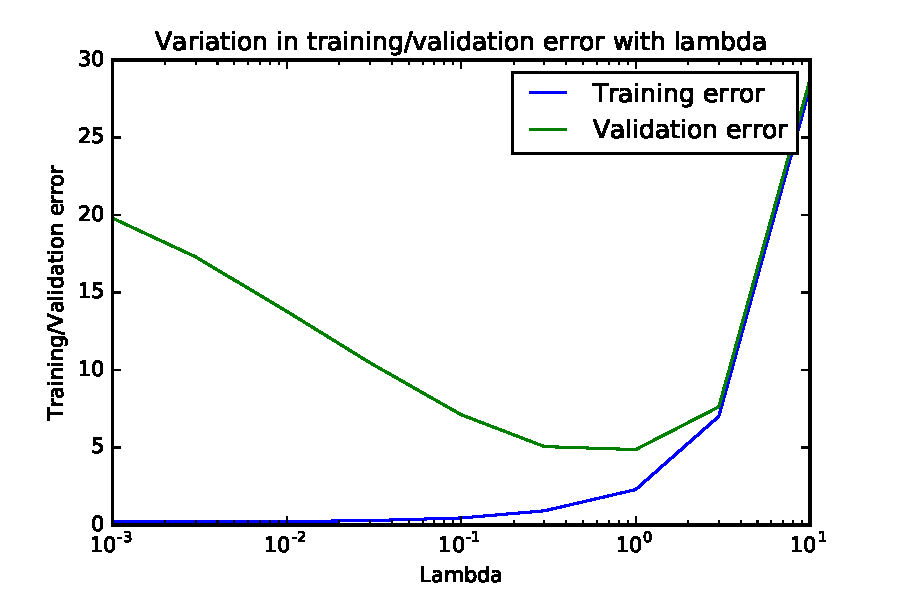
\includegraphics[scale=0.55]{part2/fig12.pdf}
\end{figure}

\begin{figure}[H]
\caption{Averaged Learning curve}
  \label{fig:avglearn}
  \centering
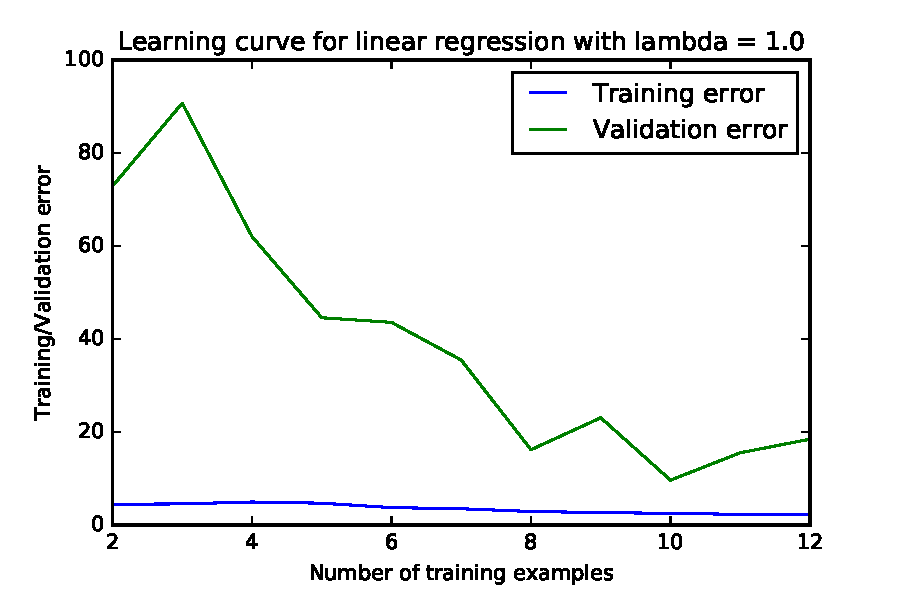
\includegraphics[scale=0.55]{part2/fig11.pdf}
\end{figure}
\fi

\end{document}